\chapter{Implementierung} \label{sec:Implementierung}

Um eine faire Vergleichbarkeit in der Umfrage zwischen den Visualisierungen zu gewährleisten, werden die Visualisierungen für diese Arbeit einheitlich implementiert. Dieses Kapitel beschreibt zunächst die Implementierung sowie die gemeinsamen Grundlagen aller Visualisierungen. Anschließend wird die Implementierung der einzelnen Visualisierungstypen erläutert.

Es werden die fünf bestplatzierten Visualisierungen aus dem Vergleich der Visualisierungen implementiert (siehe Tabelle \ref{tab:visEval_full}). Dabei wird kein Visualisierungstypen doppelt ausgewählt. Die Auswahl lautet:
\begin{enumerate}
    \setlength{\itemsep}{0pt}
    \setlength{\parskip}{0pt}
    \setlength{\parsep}{0pt}
    \item \textbf{Treemap}
    \item \textbf{Streetmap}
    \item \textbf{CodeCity}
    \item \textbf{Sunburst}
    \item \textbf{Circlular Treemap}
\end{enumerate}

\section{Gemeinsamkeiten und Architektur} \label{sec:Architektur}

Alle der ausgewählten Visualisierungen sind 2.5D-Visualisierungen. Jede Visualisierung besitzt ein eigenes Layout, das in die dritte Dimension extrudiert wird. Dabei werden drei Metriken kodiert. Eine Metrik wird über die Fläche abgebildet, eine über die Höhe und eine über die Farbe.

Die 2D-Layouts variieren hinsichtlich Form, Platzierung und Abständen, basiert jedoch alle auf einem einheitlichen Schema, welches hier definiert wird (siehe Listing \ref{lst:nodeLayoutSchema}). Im Vergleich zum Eingabe-Daten-Schema \ref{lst:nodeSchema} aus Abschnitt \ref{sec:Anwendungsfall} sind die Attribute x, y, width und length hinzugekommen, welche das Layout eindeutig beschreiben.

\begin{lstlisting}[language=json, caption={Layout-Knotenschema}, label={lst:nodeLayoutSchema}]
    "node": {
        "name": string,
        "x": number,
        "y": number,
        "width": number,
        "length": number,
        "children": List[Node] | "values": number[3]
    }
\end{lstlisting}

Die Implementierung ist bei jeder Visualisierung in zwei Schritte getrennt:
\begin{enumerate}
    \item \textbf{Layoutschritt:} In diesem Schritt wird das 2D-Layout basierend auf den Eingabedaten erzeugt. Dabei wird das Layout-Schema \ref{lst:nodeLayoutSchema} befüllt.
    \item \textbf{Visualisierungs-Schritt:} In diesem Schritt wird das generierte 2D-Layout in eine 2.5D-Visualisierung auf Basis einer Metrik in die Höhe extrudiert.
\end{enumerate}

Die Implementierung erfolgt in TypeScript mit der 3D-Rendering-Bibliothek \textit{three.js}~\cite{threejs}.

Alle Visualisierungen haben die gleichen Einstellmöglichkeiten, was Farben, Höhen, Perspektiven und Metriken betrifft.
Die Farbgebung folgt einer kontinuierlichen Skala über die Farben grün für gute Werte, gelb für mittlere Werte und rot für schlechte Werte. 
Ordner werden grau eingefärbt und erhalten umso tiefer sie sind hellere grau Töne. Dadurch können Ordner klar von Dateien ab.
Ordner werden zudem mit einer festen Extrusionshöhe versehen.





\section{Treemap} \label{sec:TreemapImplementierung}

\subsection*{Layoutschritt}
Das Treemap-Layout wird für die Visualisierung von Softwarequalitätsmetriken am häufigsten verwendet. Zudem ist es die Grundlage für alle CodeCity-Visualisierungen und hat im Vergleich der Visualisierungen am besten abgeschnitten (siehe Tabelle \ref{tab:visEval_full}). Trotzdem hat das klassische Treemap-Layout einige Nachteile und Probleme, wie in Abschnitt \ref{sec:TreemapProbleme} gezeigt werden wird. 
Aus diesen Gründen wird das Treemap-Layout in dieser Arbeit exemplarisch nicht nur implementiert, sondern auch optimiert, um zu zeigen, dass die generelle Optimierung von Layout-Algorithmen für das spezifische Anwendungsgebiet dieser Arbeit sinnvoll ist und zu besseren Ergebnissen führen kann. 
In Abschnitt \ref{sec:VerbesserungenTreemap} werden die vorgenommenen Verbesserungen beschrieben und evaluiert.

Der Output des Layoutschritts beschreibt die Position der linken unteren Ecke des Rechtecks mit den x und y Parametern sowie die Breite in x-Richtung und die Länge in y-Richtung. Bereits im Layoutschritt wird bei dieser Visualisierung Platz für Beschriftungen reserviert (siehe Abschnitt \ref{sec:BeschriftungKnoten}).

\subsection*{Visualisierungs-Schritt}
Der Visualisierungs-Schritt extrudiert alle Nicht-Blattknoten um einen festen Wert und alle Blattknoten entsprechend der Höhen-Metrik. Die z-Position jedes Knotens ergibt sich aus der z-Position des Elternknotens zuzüglich dessen Höhe. Die Fläche für die Beschriftung ist bereits im Layoutschritt reserviert worden. Die Beschriftungen werden zentral auf diesen Flächen positioniert und so skaliert, dass die Schriftgröße genau in den dafür reservierten Platz passt, ohne diesen horizontal oder vertikal zuüberschreiten. 
Ein Beispiel ist in Abbildung \ref{fig:treemapBeispielImplementierung} dargestellt.

\begin{figure}[htbp]
    \centering
    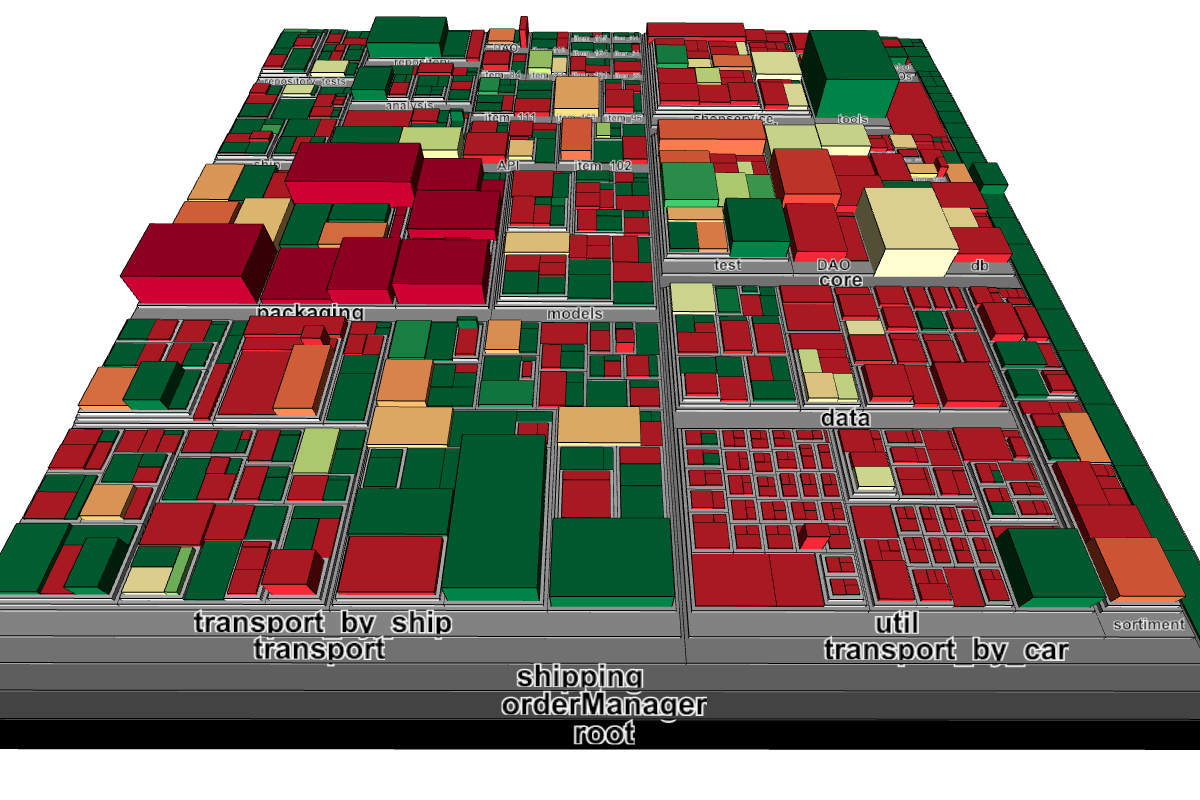
\includegraphics[width=0.7\textwidth]{images/umfrage/treemap/dreierKombi.png}
    \caption[Beispiel für Treemap-Implementierung]{Beispiel für Treemap-Implementierung, wie sie auch in der Umfrage verwendet wird.}
    \label{fig:treemapBeispielImplementierung}
\end{figure}






\section{Streetmap}

\subsection*{Layoutschritt}
Als Streetmap-Layout-Algorithmus wird der Algorithmus von dem Open Source Tool \textit{CodeCharta} verwendet~\cite{code_charta_github}. Der Algorithmus ist ein Packing-Algorithmus, der die Knoten beginnend mit den tiefsten Knoten der Struktur platziert. Dadurch resultieren, gleiche Strukturen immer in den gleichen Layouts unabhängig von deren Platzierung.

\subsection*{Visualisierungs-Schritt}
Der Output des Layoutschritts entspricht dem der Treemap, sodass ein ähnlicher Visualisierungs-Schritt eingesetzt werden kann. Der Unterschied ist, dass alle Knoten auf der Höhe von Null liegen. Die Bezeichnungen der Ordner werden mittig in der Straße platziert und so groß wie möglich gerendert, ohne andere Knoten zu schneiden. 
Ein Beispiel ist in Abbildung \ref{fig:streetmapBeispielImplementierung} dargestellt.

\begin{figure}[htbp]
    \centering
    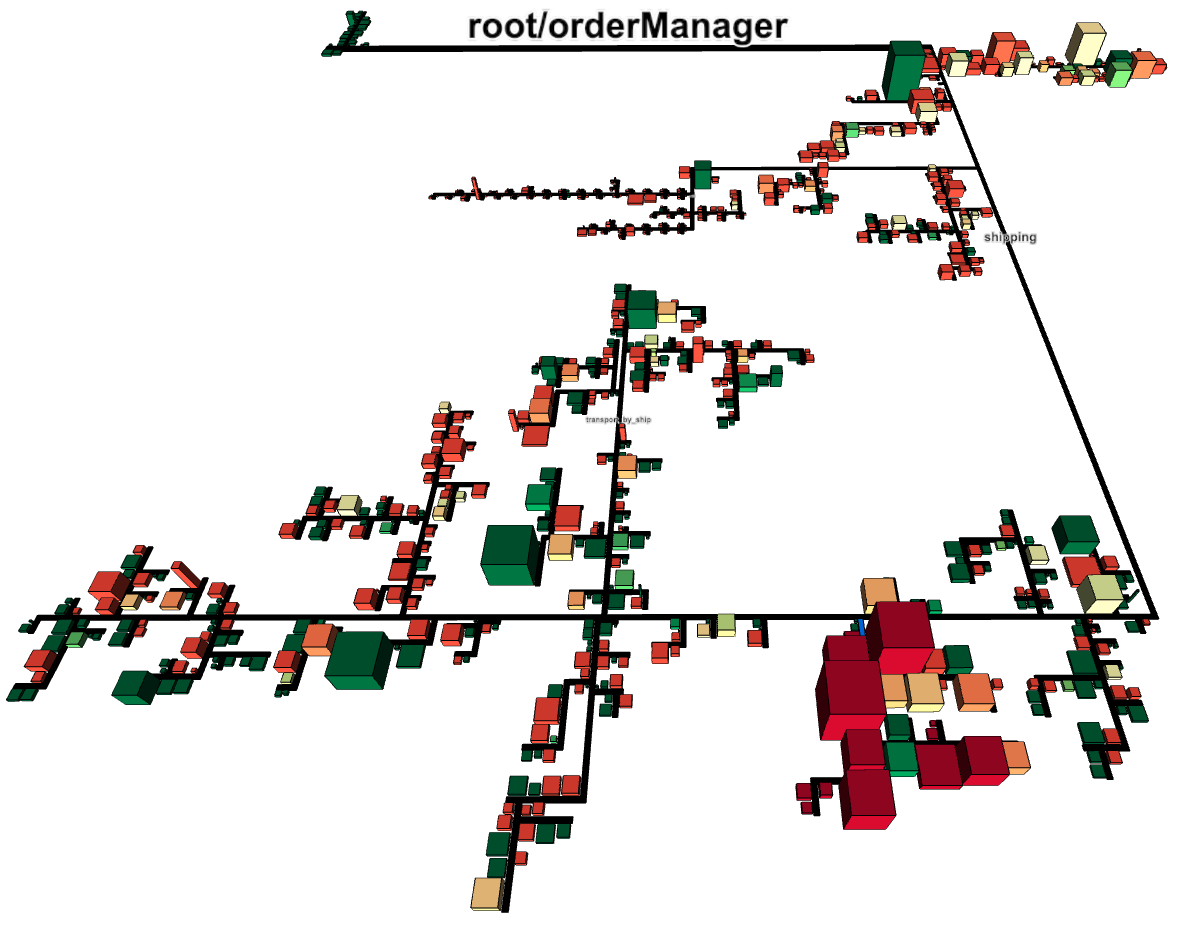
\includegraphics[width=0.7\textwidth]{images/umfrage/streetmap/dreierKombi.png}
    \caption[Beispiel für Streetmap-Implementierung]{Beispiel für Streetmap-Implementierung, wie sie auch in der Umfrage verwendet wird.}
    \label{fig:streetmapBeispielImplementierung}
\end{figure}






\section{CodeCity}

\subsection*{Layoutschritt}
Eine offene Implementierung des CodeCity-Layouts liegt nicht vor. Die Implementierung orientiert sich daher an der Beschreibung in der Originalarbeit~\cite{codeCity1}. Der Algorithmus ist ein Packing-Algorithmus, der die Knoten anders als der Splitting-Algorithmus des Treemap-Layouts, beginnend mit den tiefsten Knoten der Struktur platziert. Dadurch resultieren, wie beim Streetmap-Layout auch, gleiche Strukturen immer in den gleichen Layouts unabhängig von deren Platzierung. Die Knoten sind alle Quadrate, die von groß nach klein möglichst weit unten links positioniert werden. Bei der Platzierung wird darauf geachtet, dass die Elterknoten eine möglichst kleine Fläche haben. Dazu werden mehrere geeignete Positionen geprüft und die beste Position ausgewählt.

\subsection*{Visualisierungs-Schritt}
Da der Output des Layoutschritts dem des Treemap-Layoutschritts entspricht, wird derselbe Visualisierungs-Schritt verwendet. Ein Unterschied besteht in der Beschriftung, für die im Layoutschritt kein eigener Platz reserviert wurde. Stattdessen werden die Beschriftungen in die ohnehin vorhandenen freien Flächen im rechten oberen Teil der Knoten gesetzt und so groß wie möglich skaliert, ohne andere Knoten zu schneiden oder über die Knotenfläche hinauszuragen.
Die Implementierung ist unter folgendem \href{https://github.com/BenediktMehl/master-thesis/tree/main/anhang}{Link}\cite{anhaenge_github} verfügbar.
Ein Beispiel ist in Abbildung \ref{fig:codecityBeispielImplementierung} dargestellt.

\begin{figure}[htbp]
    \centering
    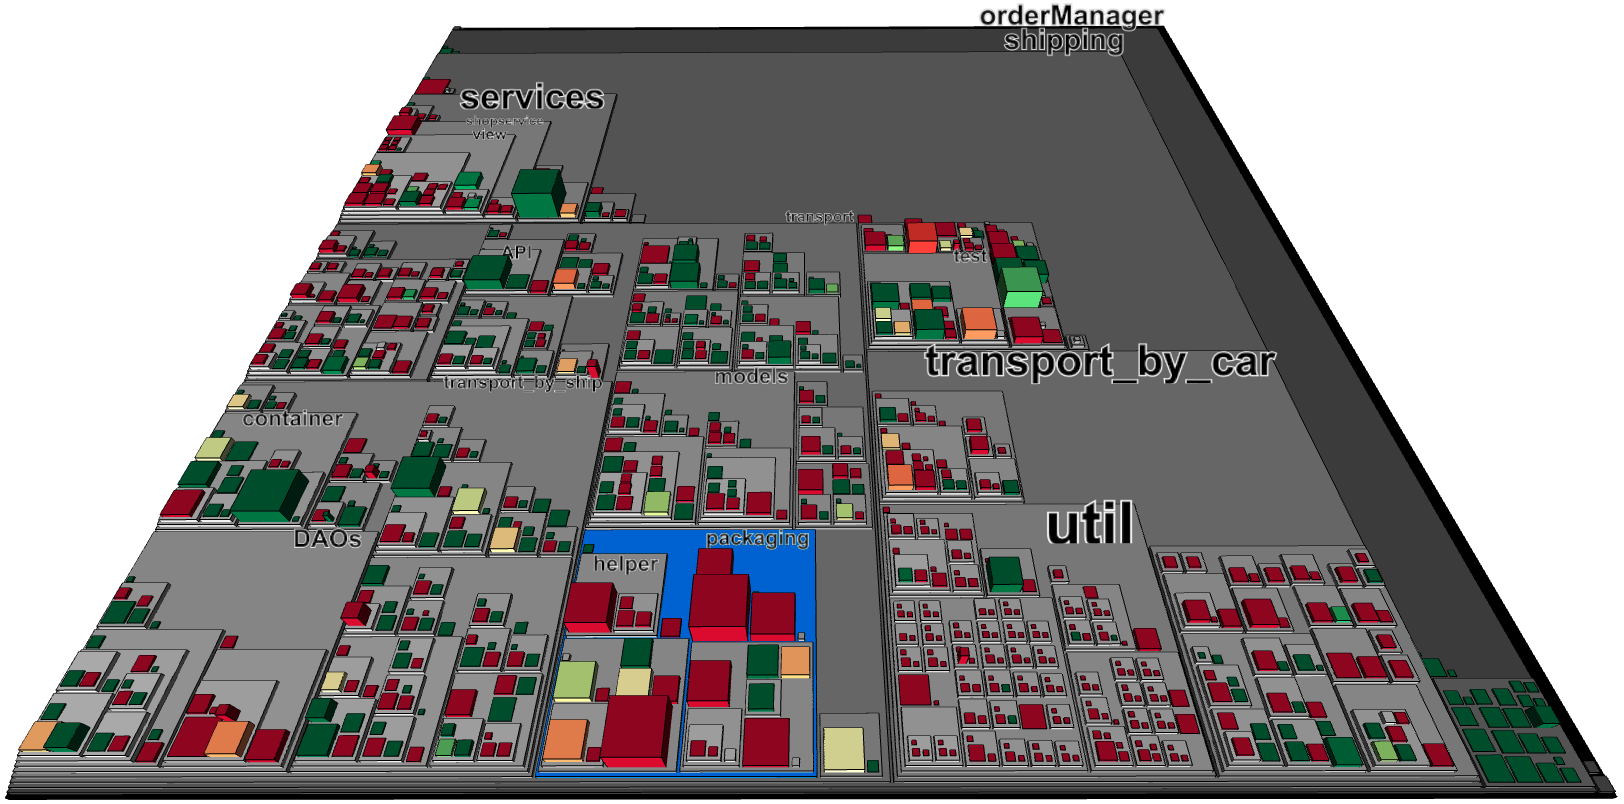
\includegraphics[width=0.7\textwidth]{images/umfrage/codecity/dreierKombi.png}
    \caption[CodeCity-Visualisierung dieser Arbeit]{CodeCity-Visualisierung dieser Arbeit}
    \label{fig:codecityBeispielImplementierung}
\end{figure}




\section{Sunburst}

\subsection*{Layoutschritt}
Zunächst werden die 360 Grad des Wurzelknotens proportional anhand der Werte der Kindknoten verteilt. Jeder Knoten erhält einen x-Wert als Startwinkel im Kreis sowie einen Breitenwert als Winkelbreite des Segments. Dieser Prozess wird rekursiv auf die Kindknoten angewendet, wobei jeweils Winkelbreite des Elternknotens auf die Kinder verteilt wird. Die y-Position und die Länge werden für dieses Layout nicht benötigt. Sie ergeben sich implizit aus der Hierarchietiefe, die den Ring bestimmt.

\subsection*{Visualisierungs-Schritt}
Der Visualisierungs-Schritt rendert die Knoten als Kreissegmente. Die z-Position resultiert aus der Hierarchietiefe. Der Radius jedes Levels also die Dicke der Segmete ist fest vorgegeben. Die Beschriftungen werden mittig im Segment mit fester Schriftgröße platziert. Die Beschriftungen können über die Segmentkanten hinausragen. Ob ein Ordner eine Beschriftung erhält, hängt von seiner effektiven Breite ab. Diese ergibt sich aus der Größe des Winkelabschnitts und aus der Position im Kreis.
Die Implementierung ist unter folgendem \href{https://github.com/BenediktMehl/master-thesis/tree/main/anhang}{Link}\cite{anhaenge_github} verfügbar.
Ein Beispiel ist in Abbildung \ref{fig:sunburstBeispielImplementierung} dargestellt.

\begin{figure}[htbp]
    \centering
    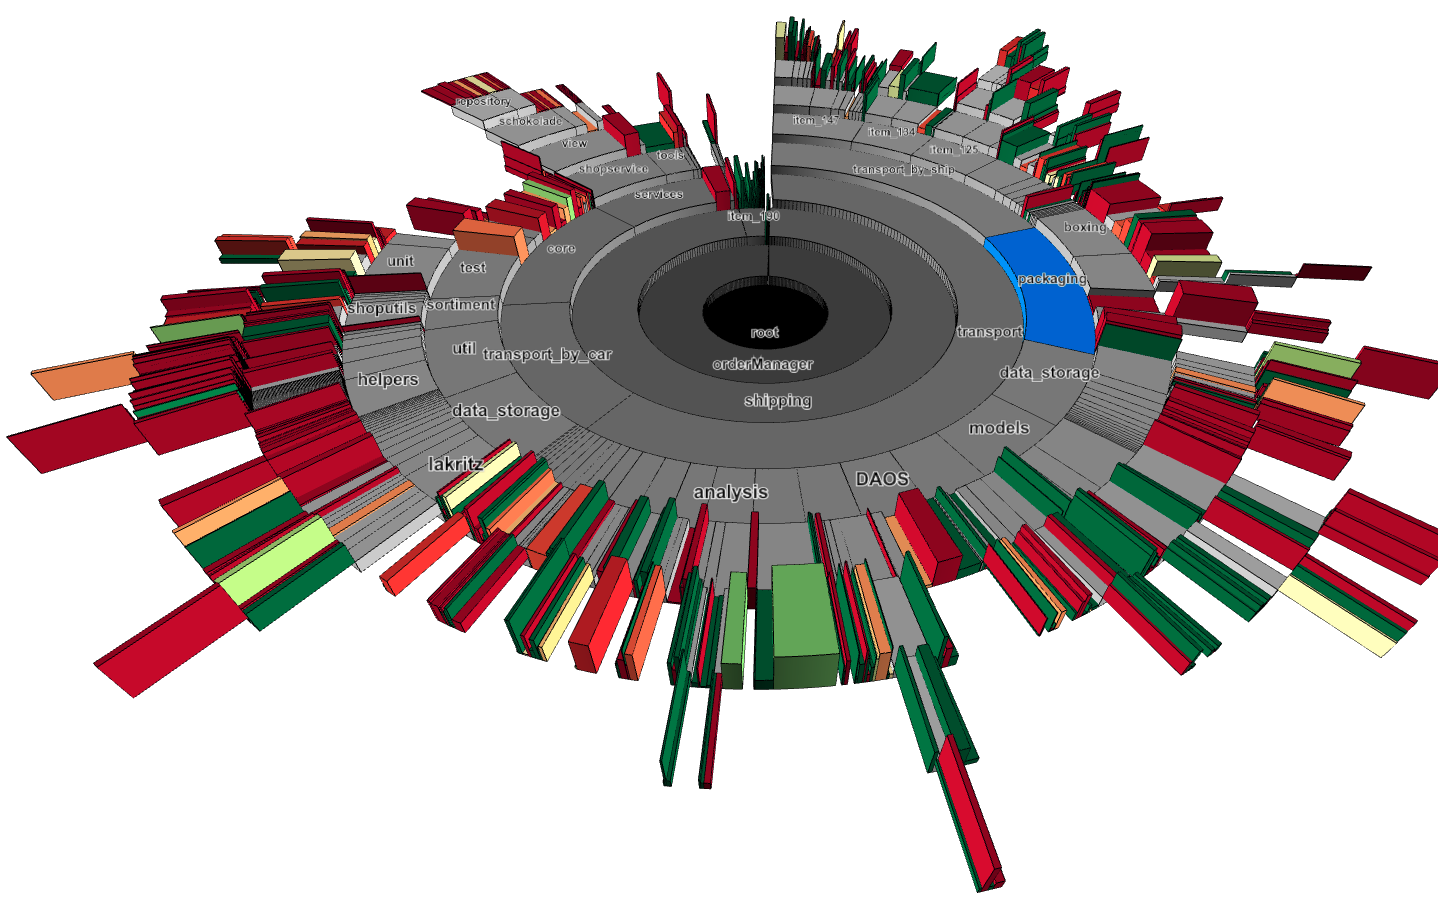
\includegraphics[width=0.7\textwidth]{images/umfrage/sunburst/dreierKombi.png}
    \caption[Sunburst-Implementierung]{Sunburst-Visualisierung dieser Arbeit}
    \label{fig:sunburstBeispielImplementierung}
\end{figure}




\section{Circular Treemap}


\subsection*{Layoutschritt}
Der Layoutschritt basiert auf dem von d3.js bereitgestellten Circle-Packing-Algorithmus~\cite{d3_treemap_doku}. Dessen Output wird in das hier definierte Schema überführt. Dabei geben x und y die Position des Kreiszentrums an und die Breite den Durchmesser des Kreises. Die Länge wird nicht verwendet.

\subsection*{Visualisierungs-Schritt}
Der Visualisierungs-Schritt entspricht weitgehend dem der Treemap. Der Unterschied liegt in der Geometrie. Knoten sind Kreise und werden zu Zylindern extrudiert. Im Layoutschritt wird kein Platz für Beschriftungen reserviert. Stattdessen werden die Beschriftungen, ähnlich wie bei CodeCity, in freien Bereichen der Kreise platziert. Beschriftungen können aus dem eigenen Knoten herausragen, sofern sie keine anderen Knoten schneiden. Dafür werden mehrere Positionen innerhalb des Kreises geprüft, um eine geeignete Lage zu finden. Die Schriftgröße wird so gewählt, dass der Text keine Überschneidungen mit anderen Knoten erzeugt.
Ein Beispiel ist in Abbildung \ref{fig:circlepackingBeispielImplementierung} dargestellt.

\begin{figure}[htbp]
    \centering
    
\includegraphics[width=0.7\textwidth]{images/umfrage/circlepacking/dreierKombi.png}
    \caption[Circle-Packing-Implementierung]{Circle-Packing-Visualisierung dieser Arbeit}
    \label{fig:circlepackingBeispielImplementierung}
\end{figure}